% Klassifiziert den Dokumenten-Typ
% Doku: http://exp1.fkp.physik.tu-darmstadt.de/tuddesign/
% Farben: http://www.tu-darmstadt.de/media/medien_stabsstelle_km/services/medien_cd/das_bild_der_tu_darmstadt.pdf
%  bigchapter: Chapter haben doppelte Schriftgröße
%  linedtoc: Linien im Inhaltsverzeichnis wie bei Überschriften
%  colorbacktitle: Der Dokumenten-Titel wird mir der Accentfarbe hinterlegt
\documentclass[bigchapter,colorback,accentcolor=tud4b,linedtoc,11pt]{tudreport}

% Input Dokument hat das Encoding UTF-8
\usepackage[utf8]{inputenc}
% Wichtiges Paket für Links und verlinktes Inhaltsverzeichnis
\usepackage[ngerman]{hyperref}
% Paket für Fußnoten
\usepackage[stable]{footmisc}
\usepackage{multirow}
\usepackage{colortbl}
% Alternatives package für bilder
\usepackage{wrapfig}
% Paket für amsmath (aligned mathe formeln)
\usepackage{amsmath}
% Farbige tabellen
\usepackage{colortbl}
 
% Paket für Bibliotheks-Verzeichnis, square: Verwende eckige statt runde klammern
% \usepackage[square]{natbib}
% Paket zum Plotten von Datensätzen
\usepackage{pgfplots}
\pgfkeys{%
  /pgfplots/seperators/.style={%
    /pgf/number format/use comma
  },
  /pgfplots/default/.style={%
    /pgf/number format/use comma,
    legend pos=north west,
    x tick label style={/pgf/number format/1000 sep=},
    y tick label style={/pgf/number format/1000 sep=},
    width=0.9\linewidth,
    height=0.40\linewidth,
    scale only axis,
    tick align=outside,
    tickpos=left,
    grid=both,
    tick align=outside,
    minor x tick num=3,
    minor y tick num=4,
    minor grid style={dotted,thin}
  }
}

% Anhänge für Original-Messdaten
\usepackage{fancyvrb}

% Verwende deutsche Bezeichner für Inhaltsverzeichnis, ... (ngerman = New German: neue Rechtschreibung)
\usepackage{ngerman}
% Deutsche Zahlen (entfernt z.B. das Leerzeichen nach einem Dezimal-Komma)
\usepackage{ziffer} 

\usepackage[verbose]{placeins}

%wegen Grafikverschiebung hinzugefügt
\usepackage{float}

%\usepackage{graphicx}
%\usepackage{caption}
\usepackage{subcaption} %Für subfigures

% PDF-Optionen
\hypersetup{%
  pdftitle={TU Darmstadt \- Physikalisches Praktikum für Fortgeschrittene},
  pdfauthor={Esra Bauer, Sören Link},
  pdfsubject={Versuch 2.2-A},
  pdfview=FitH,
}
% Nummeriere formeln in Subsections einzeln
% Kleines makro zur assymetrischen Fehlerangabe

% Entspricht-Zeichen
\usepackage{scalerel}

\newcommand\equalhat{%
\let\savearraystretch\arraystretch
\renewcommand\arraystretch{0.3}
\begin{array}{c}
\stretchto{
    \scalerel*[\widthof{=}]{\wedge}
    {\rule{1ex}{3ex}}%
}{0.5ex}\\ 
=%
\end{array}
\let\arraystretch\savearraystretch
}
%BEGINN TITELSEITE

\title{Interaction of $\gamma$-Radiation with Matter}

\subtitle{Esra Bauer  \\Sören Link}

\subsubtitle{Tutor: Haridas Pai \hfill 4/27/2015}

\author{Esra Bauer, Sören Link, Christian Hoch}

%\settitlepicture{img/title.jpg}

\institution{Physikalisches Praktikum \\für Fortgeschrittene \\ Versuch 2.2-A}

\date{\today}
%ENDE TITELSEITE


\begin{document}
%ANFANG DOKUMENT

%Titelseite einfügen
\maketitle

%Inhaltsverzeichnis einfügen
\tableofcontents

%ANFANG INHALT
\chapter{Introduction}
In this experiment we analyze the radioactive Isotopes $^{22}Na$ and
$^{137}Cs$. This includes determining the convection coefficient $\alpha_K$ of
$^{137}Cs$ and the $\beta^+$ branching coefficient of $^{22}Na$.

\chapter{Theoretical Background}
\section{Radioactice Decay}

Additionally to the well known $\alpha$, $\beta^{\pm}$ and $\gamma$ decay there are two other radioactive decay types which are important for us. First we have electron capture which gives the same progeny as $\beta^+$ decay. The nucleus absorbs an inner atomic electron whereby a proton is converted into a neutron and an electron neutrino. Released energy is given to the neutrino as kinetic energy resp.\ the progeny stays in an excited state if energy is left over. Because the missing electron is replaced by other atomic electrons there is spontaneous X-ray emission.

Second there is the inner conversion as an alternative to $\gamma$ decay. Via direct elektromagnetic interaction energy is transferred from the nucleus to an atomic electron. The nucleus switches into an lower state and the electron is emitted i.e.\ the atom is ionized. As a characteristic number we define the conversion rate as follows

$$\alpha = \frac{N_{e^-}}{N_{\gamma}}$$

where $N_{e^-}$ is the number of emitted conversion electrons and $N_{\gamma}$ is the number of emitted photons.

Below we see the decay schemes of the used Isotopes:

\begin{figure}[H]
    \centering
    \begin{subfigure}[H]{0.44\textwidth}
        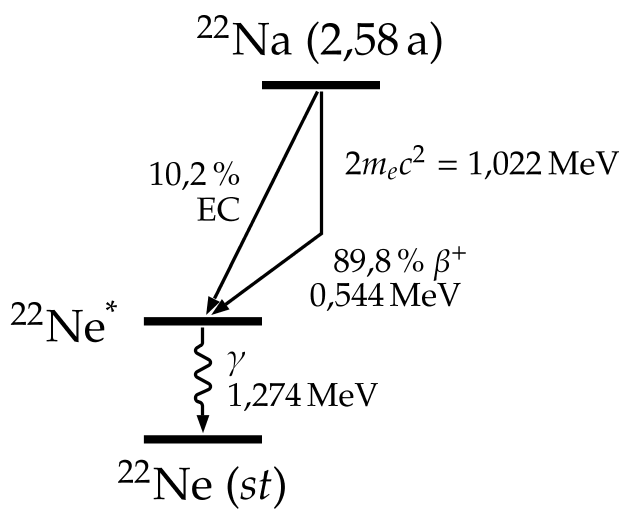
\includegraphics[width=\textwidth]{img/termschema_na22.png}
        \caption{Decay scheme of $^{22}Na$ \cite{na22decay}.}
        \label{fig:gull}
    \end{subfigure}%
    \qquad
    ~%add desired spacing between images, e. g. ~, \quad, \qquad, \hfill etc.
        %(or a blank line to force the subfigure onto a new line)
    \begin{subfigure}[H]{0.44\textwidth}
        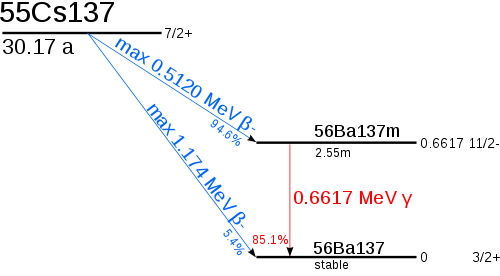
\includegraphics[width=\textwidth]{img/Cs-137-decay.png}
        \caption{Decay scheme of $^{22}Na$ \cite{cs137decay}.}
        \label{fig:tiger}
    \end{subfigure}
    \caption{Decay scheme of the radiactive isotopes used in this experiment.}
\end{figure}

\section{Interaction of $\gamma$-rays with Matter}
The interaction of $\gamma$-rays with matter consists of a superposition
of three different effects. At low photon energies their interaction with matter
is dominated by the photoelectric effect where photons are completely absorbed
by electrons. Bound electrons that absorb a photon in this way are broken free
from their atom, creating an electric current.

Photons with energies in orders of magnitudes ranging from $10^2$ $keV$ to $10^3$ $keV$
mostly interact through elastic scattering with weakly bound electrons. This
results in a transfer of energy from the photon to the electron and is called
the Comtpon effect.

Above energies of $1022keV$ photons traveling in a strong coloumb field can
spontanously convert into an electron and a positron. In doing so the photon
ceases to exists and converts it's energy first into the mass of the $e^-$ and
$e^+$ particle. The remaining energy is then being transferred onto these
particles in the form of kinetic energy. Because the impulse has to be conserved
during this conversion, the effect most often occurs near the nucleus, which can
absorb the impulse of the incident photon. This effect is called pair production
and the likelyhood of it occuring increases with higher photon energies.



\section{Scintillation Spectroscopy}

Because gamma-ray sources produce characteristic spectra with discrete lines it can be used for spectroscopy. We use a scintillation detector which operates as follows. Gamma-rays hit a thallium-doped sodium iodide (NaI) crystal which produces in consequence intense bursts of light. Those flashes unleash electrons at a photocathode which are subsequently multiplied in a photomultiplier tube. This results in an electrical pulse containing meaningful information about the particle that originally hit the detector.

Characteristic numbers for such an detector are the energy resolution and the sensitivity. Energy resolution means the smallest distance between two peaks that can still be identyfied as separate. Due to the high density scintillator its energy resolution is quite good resp.\ better than the resolution of a Geiger-müller counter but not good as that of an semiconductor detector. The sensitivity is defined as the probability for the detection of a particle. Especially in case of inorganic scintillation crystals as used in this experiment, the sensitivity for charged particles is very high due to the use of the phomultiplier tube.

The pulse height spectrum is the distribution of various pulse strenghts (heights) developed while recording the gamma-ray spectrum. The pulse heights are digitized and saved in channels for later spectral analysis.

\chapter{Experimental Setup and Execution}
\begin{figure}[H] 
  \centering
     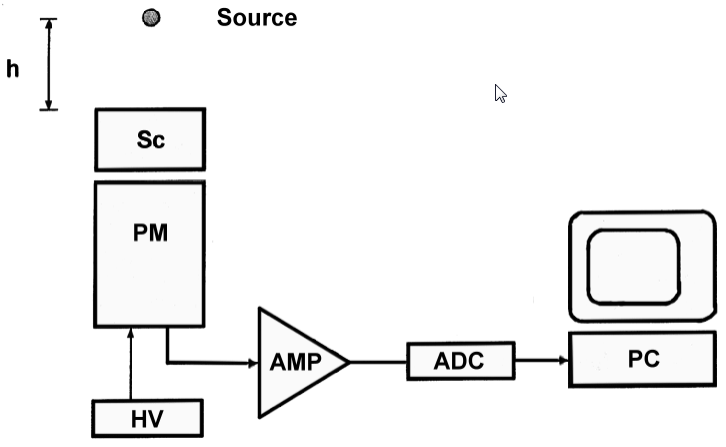
\includegraphics[width=0.8\textwidth]{img/aufbau.png}
     \caption{Experimental setup. As source material we used $^{22}Na$ and
       $^{137}Cs$. In addition we mounted plates of aluminium, cadmium, iron and
     lead behind the source to measure the backscatter radiation. Finally we have
     also measured the background radiation without a radiactive source \cite{Anleitung}.}
  \label{fig:aufbau}
\end{figure}

The experimental setup remains mostly constant throughout the experiment. First
we measured the radioactive spectrum of $^{137}Cs$ with a distance $h$ from the
detecter of $10 cm$. During these measurements
we mounted plates of aluminium, cadmium, iron and lead behind the source to
determine their effect on the spectrum. We've also measured the spectrum of
$^{137}Cs$ through a lead shield.

Afterwards we replaced the caesium isotope with radioactive $^{22}Na$ and
measured it's spectrum twice. The first measurement was done with the natrium
sample mounted $10 cm$ above the scintillation detector. For the second
measurment we put the sample directly on top of the detector.

Each measurement concluded when the main peak of the spectrum reached $3000$ counts.

In the end we measured the background radiation for 31 minutes and 40 seconds.

\chapter{Evaluation}
\section{Analysis of the spectrum of $^{137}Cs$}
\subsection{Energy-calibration}
\begin{center}
\begin{figure}[H]
    \begin{tikzpicture}
    \begin{axis}[
        title={$^{137}Cs$ Spectrum},
        xlabel=channel,
        ylabel=counts,
        height=0.7\textwidth,
        ymin=0,
        xmin=0,
        xmax=320,
        default
    ]
    \addplot[red, only marks, mark=x, mark size=1pt] table[x index=0, y index=1] {data/Cs137-1-no-bg.txt};
    \addplot[green, mark=x, mark size=0pt, samples=100, domain=-60:115, thick] {1850.15*e^(-0.037403*(-90.6604+x)^2)};
    \addlegendentry{X-ray peak fit}
    \addplot[blue, mark=x, mark size=0pt, samples=100, domain=190:270, thick] {4367.33*e^(-0.00790729*(-232.226+x)^2)};
    \addlegendentry{Gamma-ray peak fit}
    \end{axis}
    \end{tikzpicture}
    \captionof{figure}{}
\end{figure}
\end{center}

\subsubsection{Fit Values}

$$f(x) = k\cdot \frac{1}{\sqrt{2 \pi } \sigma} \cdot e^{-\frac{(x-\mu )^2}{2 \sigma ^2}}$$

\begin{center}
  \begin{tabular}{r|r|r|r|r|r|r}
           & $k$     & $\Delta k$ & $\mu$   & $\Delta \mu$ & $\sigma$ & $\delta \sigma$ \\ \hline
     xray  & $16956$ & $303$      & $90,7$  & $0,07$       & $3,66$   & $0,08$          \\ \hline
     gamma & $87052$ & $2603$     & $232,2$ & $0,27$       & $7,95$   & $0,28$          \\
	\end{tabular}
\end{center}


\subsection{Energy spectrum}

\subsection{Backscattering peak}
\begin{center}
\begin{figure}[H]
    \begin{tikzpicture}
    \begin{axis}[
        title={$^{137}Cs$ Spectrum},
        xlabel=channel,
        ylabel=counts,
        height=0.7\textwidth,
        ymin=0,
        xmin=0,
        xmax=320,
        default
    ]
    \addplot[red, only marks, mark=x, mark size=1pt] table[x index=0, y index=1] {data/Cs137-AL-backscattering-no-bg.txt};
    \addlegendentry{Aluminium Plate}
    \addplot[green, only marks, mark=x, mark size=1pt] table[x index=0, y index=1] {data/Cs137-Cd-backscattering-no-bg.txt};
    \addlegendentry{Cadmium Plate}
    \addplot[blue, only marks, mark=x, mark size=1pt] table[x index=0, y index=1] {data/Cs137-Fe-backscattering-no-bg.txt};
    \addlegendentry{Iron Plate}
    \addplot[orange, only marks, mark=x, mark size=1pt] table[x index=0, y index=1] {data/Cs137-Pb-backscattering-no-bg.txt};
    \addlegendentry{Lead Plate}
    \end{axis}
    \end{tikzpicture}
    \captionof{figure}{}
\end{figure}
\end{center}

\subsection{Abosrption by a lead plate}
\begin{center}
\begin{figure}[H]
    \begin{tikzpicture}
    \begin{axis}[
        title={$^{137}Cs$ Spectrum},
        xlabel=channel,
        ylabel=counts,
        height=0.7\textwidth,
        ymin=0,
        xmin=0,
        xmax=320,
        default
    ]
    \addplot[red, only marks, mark=x, mark size=1pt] table[x index=0, y index=1] {data/Cs137-1-no-bg.txt};
    \addlegendentry{Without lead plate}
    \addplot[red, only marks, mark=x, mark size=1pt] table[x index=0, y index=1] {data/Cs137-Pb-shield-no-bg.txt};
    \addlegendentry{With lead plate}
    \end{axis}
    \end{tikzpicture}
    \captionof{figure}{}
\end{figure}
\end{center}
\subsection{Convection coefficient}

\section{Analysis of the spectrum of $^{22}Na$}
\subsection{Energy-calibration}
\begin{center}
\begin{figure}[H]
    \begin{tikzpicture}
    \begin{axis}[
        title={$^{22}Na$ Spectrum},
        xlabel=channel,
        ylabel=counts,
        height=0.7\textwidth,
        ymin=0,
        xmin=0,
        xmax=320,
        default
    ]
    \addplot[red, only marks, mark=x, mark size=1pt] table[x index=0, y index=1] {data/Na22-no-bg.txt};
    \addplot[green, mark=x, mark size=0pt, samples=150, domain=100:220, thick] {5344.67*e^(-0.0359942*(-145.464+x)^2)};
    \addlegendentry{Annihilation peak fit}
    \addplot[blue, mark=x, mark size=0pt, samples=100, domain=190:270, thick] {963.17*e^(-0.0180637*(-235.828+x)^2)};
    \addlegendentry{Second peak fit}
    \end{axis}
    \end{tikzpicture}
    \captionof{figure}{}
\end{figure}
\end{center}

\subsubsection{Fit Values}
\begin{center}
  \begin{tabular}{r|r|r|r|r|r|r}
                   & $k$     & $\Delta k$ & $\mu$   & $\Delta \mu$ & $\sigma$ & $\delta \sigma$ \\ \hline
     annihilation  & $49932$ & $2597$     & $145,5$  & $0,22$       & $3,73$   & $0,22$          \\ \hline
     photo         & $12702$ & $799$      & $235,8$  & $0,38$       & $5,26$   & $0,38$          \\
	\end{tabular}
\end{center}


\subsection{Energy spectrum}
\subsection{Probability of sumpeaks}
\begin{figure}[H]
\begin{tikzpicture}
\begin{axis}[
  default,
  width=0.48\linewidth,
  title={$^{22}Na$ Spectrum},
  xlabel=channel,
  ylabel=counts,
  height=0.3\linewidth,
  ymin=0,
  xmin=50,
  xmax=350,
  name=first
]
    \addplot[blue, only marks, mark=x, mark size=1pt] table[x index=0, y index=1] {data/Na22-no-bg.txt};
    \addplot[red, only marks, mark=x, mark size=1pt] table[x index=0, y index=1] {data/Na22-sum-no-bg.txt};

\end{axis}

\begin{axis}[
  default,
  width=0.28\linewidth,
  title={$^{22}Na$ Spectrum},
  xlabel=channel,
  ylabel=counts,
  height=0.3\linewidth,
  ymin=0,
  xmin=280,
  xmax=320,
  name=second,
  at=(first.outer south east),
  anchor=outer south west
]
    \addplot[blue, only marks, mark=x, mark size=1pt] table[x index=0, y index=1] {data/Na22-no-bg.txt};
    \addplot[red, only marks, mark=x, mark size=1pt] table[x index=0, y index=1] {data/Na22-sum-no-bg.txt};
\end{axis}
\end{tikzpicture}
\captionof{figure}{}
\end{figure}
\subsection{$\beta^+$-branching ratio}
\subsection{Multiple event process}

\section{Energy Resolution}

\section{Background Radiation}

\begin{center}
\begin{figure}[H]
\begin{tikzpicture}
\begin{axis}[
    title={Background Radiation},
    xlabel=channel,
    ylabel=counts,
    height=0.7\textwidth,
    ymin=0,
    xmin=0,
    xmax=650,
    default
]
\addplot[red, only marks, mark=x, mark size=1pt] table[x index=0, y index=1] {data/background.txt};
\end{axis}
\end{tikzpicture}
\captionof{figure}{}
\end{figure}
\end{center}

\chapter{Conclusion}

%ENDE INHALT
\cleardoublepage{}
% Eintrag fürs Inhaltsverzeichnis
\newpage
\begin{thebibliography}{100}
  \bibitem{Anleitung} {Experimental Instructions} \bibitem{na22decay} {Semibyte, homepage of physics lab assistent and qualified
      computer scientist Tobias Krähling:
      \url{http://www.semibyte.de/wp/download/graphicslib/physics/termschema_na22.png}
    [CC BY-NC-SA 3.0]}
  \bibitem{cs137decay} {Wikipedia, the free encyclopedia. By Tubas-en [Public
      domain], via Wikimedia Commons: \url{http://upload.wikimedia.org/wikipedia/commons/thumb/3/3e/Cs-137-decay.svg/500px-Cs-137-decay.svg.png}}
\end{thebibliography}
\end{document}

%%% Local Variables:
%%% mode: latex
%%% TeX-master: t
%%% End:
